\documentclass[11pt,a4paper]{article}
\usepackage{polski}
\usepackage[utf8]{inputenc}
\usepackage[colorlinks=true,linkcolor=black,urlcolor=blue,citecolor=RoyalBlue]{hyperref}
\usepackage[usenames,dvipsnames]{color}
\usepackage{alltt}
\usepackage{booktabs} % eleganckie tabelki
\usepackage{graphicx}
\usepackage{bm}		% bold math symbols

\newcounter{liczp}
\newenvironment{example}{\refstepcounter{liczp}{\noindent
{\bf Przykład~\theliczp:}\,}}

\usepackage{parcolumns}	% two-column paragraphs
\usepackage{subfigure}
\usepackage{floatrow}
% Table float box with bottom caption, box width adjusted to content
\newfloatcommand{capbtabbox}{table}[][\FBwidth]

\addtolength{\textwidth}{4cm}
\addtolength{\hoffset}{-2cm}
\addtolength{\textheight}{4cm}
\addtolength{\voffset}{-2cm}
\date {\today}
\author {
Aleksy Barcz\\
Instytut Systemów Elektronicznych
}
%\keywords{teoria wrażliwości, sieci neuronowe}

\title{\vspace{60mm} \textbf{Analiza metody uczenia sieci neuronowych wykorzystującej teorię wrażliwości} \\ sprawozdanie z pracowni naukowej}
\begin{document}
\maketitle
\thispagestyle{empty}

\newpage

\tableofcontents

\newpage

\section{Wstęp}
Sprawozdanie zawiera analizę metody szybkiego uczenia trójwarstwowych sieci neuronowych, zaproponowanej przez Enrique Castillo~\cite{castillo2006very}. Metoda wrażliwościowa powstała jako rozszerzenie \emph{metody~funkcji~odwrotnej}~\cite{castillo2002global}, służącej do uczenia sieci dwuwarstwowych, na sieci trójwarstwowe. Metoda wrażliwościowa wykorzystuje teorię wrażliwości, której zastosowanie polega na obliczeniu jak zmiana jednej zmiennej należącej do modelu wpływa na wartości pozostałych zmiennych modelu.

\section{Wprowadzenie}
Model jedno i trójwarstwowej sieci neuronowej jest modelem dojrzałym. Jednym z pierwszych algorytmów uczenia sieci neuronowej było uczenie przy użyciu \emph{reguły delta}, opierającej się na obliczeniu w jaki sposób wartości \emph{wag} sieci wpływają na błąd całkowity. Z biegiem czasu powstały sprawdzone algorytmy uczenia sieci neuronowych, takie jak LM i BFGS, pozwalające na minimalizację błędu przy użyciu aproksymacji Hesjanu a także inne metody, oparte na gradiencie bądź nie (jak np. RPROP~\cite{riedmiller1993direct}).

Wszystkie te rozwiązania posiadają jednak (w mniejszym bądź większym stopniu) pewną wadę. Wskutek wykorzystania nieliniowych funkcji aktywacji, nie będących funkcjami wypukłymi, funkcja błędu może posiadać poza minimum globalnym również minima lokalne. W szczególności zostało wykazane, że dla pojedynczego neuronu z logistyczną funkcją aktywacji funkcja błędu dla zbioru $n$ próbek o rozmiarze $d$ może posiadać $\lfloor n/d \rfloor^{d}$ minimów lokalnych~\cite{auer1996exponentially}. Może się zdarzyć że po osiągnięciu takiego minimum lokalnego, wybrana metoda uczenia sieci nie będzie potrafiła wyjść z niego, wskutek czego wynikiem uczenia mogą być lepsze lub gorsze minima funkcji błędu.

Dodatkowo, zbieżność algorytmu może wymagać dużej ilości kroków. Dobry czas uczenia, mierzony w ilości epok, potrafią uzyskać metody drugiego rzędu, takie jak LM i BFGS, jednakże dzieje się to kosztem zwiększonej złożoności obliczeniowej.

Zaproponowana przez Castillo metoda uczenia sieci neuronowych ma na celu uniknięcie tych dwóch wad. Poprzez linearyzację problemu (metoda funkcji odwrotnej) jednowarstwowa sieć neuronowa może być nauczona w jednej iteracji, z gwarancją osiągnięcia globalnego minimum. W przypadku trójwarstwowych sieci neuronowych, wykorzystano teorię wrażliwości do uproszczenia obliczeń. Jako nowy parametr modelu przyjęto wartości wyjściowe warstwy ukrytej, względem których liczone są wrażliwości funkcji błędu. Dzięki temu ilość iteracji uczenia została zmniejszona do kilku~\cite{castillo2006very}. Dodatkową korzyścią z użycia tej metody jest to, że jako produkt uboczny procesu uczenia otrzymujemy wrażliwości funkcji błędu względem poszczególnych neuronów ukrytych, czyli możemy stwierdzić który neuron wpływa najbardziej na jakość otrzymanych wyników.

Metoda wrażliwościowa nie ogranicza się jedynie do jedno i trójwarstwowych sieci neuronowych. Według jej autorów, dotychczasowa analiza wrażliwości skupiała się głównie na metodzie najmniejszych kwadratów w zastosowaniu do zadań regresji liniowej~\cite{castillo2004general}. Zaproponowali oni ogólny model nieliniowej optymalizacji, który można analizować przy użyciu teorii wrażliwości. Przykładowo można w ten sposób zanalizować zadanie typu Minimax, LAV oraz zadanie maksymalnego prawdopodobieństwa~\cite{castillo2004general}.

\newpage

\subsection{Metoda funkcji odwrotnej - wprowadzenie}
Dwuwarstwowa sieć neuronowa to sieć składająca się z warstwy wejść (neuronów wejściowych), nie wykonujących żadnych obliczeń, oraz warstwy neuronów wyjściowych - o dowolnej funkcji aktywacji. Zależność wyjść sieci $y_{js}$ od wejść $x_{is}$ można opisać wzorem~\ref{eq:cstonelayer}, gdzie $I$ - ilość wejść sieci, $J$ - ilość neuronów wyjściowych, $S$ - ilość próbek.

\begin{equation}
y_{js} = f_j \left( w_{j0} + \sum_{i=1}^{I}w_{ji}x_{is} \right); \quad j = 1,2,...,J; \quad s = 1,2,...,S.
\label{eq:cstonelayer}
\end{equation}

Dla tego układu równań poszukujemy minimum błędu kwadratowego, opisanego równaniem~\ref{eq:cstonelayerq}.
\begin{equation}
Q = \sum_{s=1}^{S} \sum_{j=1}^{J} \left( y_{js} - f_j \left( w_{j0} + \sum_{i=1}^{I}w_{ji}x_{is} \right)\right)^{2}.
\label{eq:cstonelayerq}
\end{equation}

Tak sformułowane zadanie optymalizacji, dla nieliniowych funkcji aktywacji $f_j$, wymaga użycia metod gradientowych. Metoda funkcji odwrotnej~\cite{castillo2002global} polega na zastąpieniu powyższego układu równań nieliniowych układem równań liniowych opisanym wzorem~\ref{eq:cstonelayerinv}, gdzie~$f^{-1}_j$ - funkcja odwrotna do~$f_j$. Taki układ równań można rozwiązać w jednym kroku.

\begin{equation}
f^{-1}_j(y_{js}) =  w_{j0} + \sum_{i=1}^{I}w_{ji}x_{is}; \quad j = 1,2,...,J; \quad s = 1,2,...,S.
\label{eq:cstonelayerinv}
\end{equation}


\subsection{Metoda wrażliwościowa - wprowadzenie}
W przypadku trójwarstwowych sieci neuronowych (wejścia, warstwa ukryta, warstwa wyjściowa), o nieliniowej funkcji aktywacji warstwy ukrytej, nie da się bezpośrednio przekształcić układu równań nieliniowych na układ równań liniowych. Metoda wrażliwościowa wykorzystuje teorię wrażliwości do przekształcenia podstawowego układu równań sieci neuronowej do układu równań optymalizującego inny zestaw zmiennych - $z_{ks}$. Podstawy teorii wrażliwości w zastosowaniu do problemów optymalizacji zostały przedstawione w~\cite{castillo2004general}, natomiast zastosowanie do uczenia trójwarstwowych sieci neuronowych w~\cite{castillo2006very}. Poszczególne wzory wykorzystywane przez metodę wrażliwościową zostały zaprezentowane w sekcji~\ref{sec:castillodelta}.

\subsection{Zbiory danych}
Do eksperymentów użyto dwóch zbiorów danych: prostego zadania regresji jednowymiarowej oraz wartości dziennego zamknięcia indeksu Dow Jones z lat 1994-1996 (753 próbki). Zgodność zaimplementowanej metody z metodą wrażliwościową opisaną w~\cite{castillo2006very} sprawdzono porównując wynik predykcji wartości indeksu Dow Jones na podstawie próbek z ostatnich 5ciu dni. Zastosowano architekturę sieci 5-7-1, tak samo jak w oryginalnym artykule~\cite{castillo2006very} i uzyskano wynik podobnego rzędu: $10^{-3}$ zarówno dla funkcji aktywacji neuronów ukrytych $tanh$ jak i $logsig$. Celem eksperymentów na obu zbiorach danych była minimalizacja błędu MSE na zbiorze uczącym.

\section{Metoda wrażliwościowa jako modyfikacja reguły delta~\label{sec:castillodelta}}
Zależność wyjść $y_{js}$ od wejść $x_{is}$ można dla trójwarstwowej sieci neuronowej opisać wzorem~\ref{eq:threelayer}, gdzie indeks $^{(1)}$ oznacza przynależność do warstwy ukrytej, a indeks $^{(2)}$ - do warstwy wyjściowej.

\begin{equation}
y_{js} = f^{(2)}_j \left( w^{(2)}_{j0} + \sum_{k=1}^{K} w^{(2)}_{jk} f^{(1)}_k \left( w^{(1)}_{k0} + \sum_{i=1}^{I}w^{(1)}_{ki}x_{is} \right)\right); \quad j = 1,2,...,J; \quad s = 1,2,...,S.
\label{eq:threelayer}
\end{equation}

\newpage

\noindent Tę samą zależność można opisać, wprowadzając pomocniczą zmienną $z_{ks}$, wzorami~\ref{eq:threelayer2} oraz~\ref{eq:threelayer1}.

\begin{equation}
y_{js} = f^{(2)}_j \left( w^{(2)}_{j0} + \sum_{k=1}^{K} w^{(2)}_{jk} z_{ks}\right); \quad j = 1,2,...,J; \quad s = 1,2,...,S.
\label{eq:threelayer2}
\end{equation}

\begin{equation}
z_{ks} = f^{(1)}_k \left( w^{(1)}_{k0} + \sum_{i=1}^{I}w^{(1)}_{ki}x_{is} \right); \quad k = 1,2,...,K; \quad s = 1,2,...,S.
\label{eq:threelayer1}
\end{equation}

\subsection{Reguła delta}
Łączny błąd na zbiorze $S$ próbek możemy określić wzorem~\ref{eq:sse} (SSE), gdzie $d_{js}$ to oczekiwana wartość na wyjściu $j$-ego neuronu wyjściowego dla próbki $s$.

\begin{equation}
Q = \sum_{s=1}^{S} \sum_{j=1}^{J} \left( y_{js}  - d_{js} \right)^{2}.
\label{eq:sse}
\end{equation}

W przypadku reguły delta błąd ten jest minimalizowany poprzez odpowiednią modyfikację wartości wag $w^{(1)}$ oraz $w^{(2)}$. Odpowiednie korekty $\Delta w_{n}$ są wyznaczane przy użyciu rozwinięcia $Q$ w szereg Taylora - wzór~\ref{eq:taylor} (gdzie $n$ jest indeksem każdej kolejnej wagi warstw ukrytej i wyjściowej) tak by $Q(\bm{w} + \Delta \bm{w}) = 0$.

\begin{equation}
Q(\bm{w} + \Delta \bm{w}) = Q(\bm{w}) + \sum_{n} \frac{\partial Q(\bm{w})}{\partial w_{n}} \Delta w_{n} \approx 0.
\label{eq:taylor}
\end{equation}

\subsection{Metoda wrażliwościowa}
Metoda wrażliwościowa w podobny sposób redukuje błąd SSE, tylko zamiast modyfikować bezpośrednio wagi sieci $w$, modyfikuje wartości pośrednie $z_{ks}$ na podstawie których obliczane są dopiero wartości $w^{(1)}_{ki}$ oraz $w^{(2)}_{jk}$ (układy równań liniowych). Łączny błąd tak określonego problemu wyrażony jest wzorem~\ref{eq:qall}. Składnik $Q^{(2)}$ to zwyczajny błąd SSE (po zastosowaniu przekształcenia $f_j^{(2)^{-1}}$), natomiast $Q^{(1)}$ ma na celu regularyzację wartości $z_{ks}$, tak by $z_{ks}$ stało się rzeczywistym wyjściem warstwy ukrytej.

\begin{equation}
Q = Q^{(1)} + Q^{(2)} = \sum_{s=1}^{S} \left[ \sum_{k=1}^{K} \left( \sum_{i=1}^{I} w^{(1)}_{ki} x_{is} - f^{(1)^{-1}}_k(z_{ks}) \right)^{2} + \sum_{j=1}^{J} \left( \sum_{k=1}^{K} w^{(2)}_{jk} z_{ks} - f^{(2)^{-1}}_j(d_{js}) \right)^{2} \right].
\label{eq:qall}
\end{equation}

\noindent Zamiast $\frac{\partial Q(\bm{w})}{\partial w_n}$, obliczane są wrażliwości $\frac{\partial Q(\bm{z})}{\partial z_{ks}}$, zgodnie z rozwinięciem~\ref{eq:qdz} oraz wzorem~\ref{eq:dqdz}. (Komentarz do poprawności wzoru~\ref{eq:dqdz} znajduje się w sekcji~\ref{sec:dqdzcor}.)

\begin{equation}
Q(\bm{z} + \Delta \bm{z}) = Q(\bm{z}) + \sum_{k=1}^{K}\sum_{s=1}^{S} \frac{\partial Q(\bm{z})}{\partial z_{ks}} \Delta z_{ks} \approx 0.
\label{eq:qdz}
\end{equation}

\begin{equation}
\frac{\partial Q}{\partial z_{ks}} = -\frac{2 \left( \sum_{i=1}^{I} w^{(1)}_{ki} x_{is} - f^{(1)^{-1}}_k(z_{ks}) \right)}{f'^{(1)}_k(z_{ks})} + 2 \sum_{j=1}^{J} \left( \sum_{k=1}^{K} w^{(2)}_{jk} z_{ks} - f^{(2)^{-1}}_j(d_{js}) \right) w^{(2)}_{jk}.
\label{eq:dqdz}
\end{equation}

\subsection{Porównanie}
Zastosowanie reguły delta ma charakter iteracyjny. Przy losowych wartościach początkowych wag nie jest możliwe uzyskanie minimalnej wartości błędu $Q$ w jednej iteracji, więc iteracje należy powtarzać aż do osiągnięcia satysfakcjonującego minimum. W trakcie procesu uczenia sieci, modyfikacji ulegają wagi obydwu warstw, dzięki czemu możliwe jest uzyskanie optymalnej dla danego problemu architektury sieci neuronowej.

W przypadku metody wrażliwościowej, charakter obliczeń zależy od zastosowanej metody inicjalizacji $z_{ks}$. Jeśli zastosuje się zalecaną w artykule~\cite{castillo2006very} metodę:

\begin{equation}
z_{ks} = f^{(1)}_{k} \left( \sum_{i=1}^{I} w^{(1)}_{ki} x_{is} \right).
\label{eq:zinit}
\end{equation}

\noindent można uzyskać dobrze nauczoną sieć neuronową w jednej iteracji. Niestety, wskutek takiej inicjalizacji, wartości $Q^{(1)}$ są bliskie zeru, przez co wartości $w_{ki}^{(1)}$ nie ulegają zmianie w procesie uczenia. Dopiero po kilku iteracjach (ok. 3 dla danych DJI) następują zmiany wartości $w_{ki}^{(1)}$.

W przypadku losowej inicjalizacji $z_{ks}$ (uwaga: wartości muszą być losowane z zakresu odpowiedniego dla wyjść $f_k^{(1)}$), uczenie sieci ma charakter iteracyjny - dla danych DJI wynik zbliżony do uzyskanego pierwszą metodą udało się uzyskać po ok. 10-20 iteracjach.

\section{Analiza poprawności wzorów opisujących wrażliwość}
\subsection{Odwrotność pochodnej zamiast pochodnej odwrotności funkcji\label{sec:dqdzcor}}
We wzorze~\ref{eq:dqdz} występuje błąd, powtórzony w~\cite{castillo2006very} oraz~\cite{guijarro2006new}. Zamiast pochodnej funkcji odwrotnej ${f^{(1)^{-1}}}'$ została użyta odwrotność pochodnej funkcji $\frac{1}{f'^{(1)}}$. Wartości te nie są sobie równe zarówno dla funkcji aktywacji \emph{tanh} jak i \emph{logsig}. Poprawiony wzór powinien mieć postać:

\begin{equation}
\frac{\partial Q}{\partial z_{ks}} = - 2 \left( \sum_{i=1}^{I} w^{(1)}_{ki} x_{is} - f^{(1)^{-1}}_k(z_{ks}) \right) {f^{(1)^{-1}}_k}'(z_{ks}) + 2 \sum_{j=1}^{J} \left( \sum_{k=1}^{K} w^{(2)}_{jk} z_{ks} - f^{(2)^{-1}}_j(d_{js}) \right) w^{(2)}_{jk}.
\label{eq:dqdzcor}
\end{equation}

Różnice między wartościami ${f^{(1)^{-1}}}'$ i $\frac{1}{f'^{(1)}}$ przedstawiono na wykresach~\ref{fig:finvd1} i~\ref{fig:finvd2}. Na wykresie~\ref{fig:finvd1} użyto wartości $x \in (-0.9, 0.9)$ jako poprawnych wartości wyjściowych funkcji aktywacji $tanh(x)$, natomiast na wykresie~\ref{fig:finvd2} użyto wartości $x \in (0.1, 0.9)$ jako poprawnych wartości wyjściowych funkcji aktywacji $logsig(x)$. Poprawne funkcje ${f^{(1)^{-1}}}'$ charakteryzują się znacznie większymi wartościami na skrajach przedziałów.

\begin{figure}[h!]
\begin{floatrow}
\ffigbox[\FBwidth]{	% use the image width
	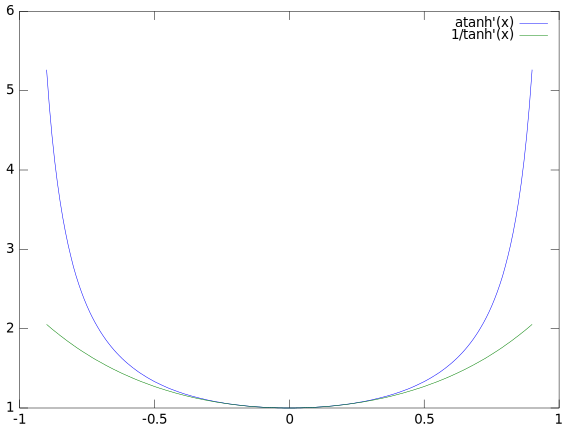
\includegraphics[scale=0.45]{tanh}
}{
\caption{${f^{(1)^{-1}}}'$ i $\frac{1}{f'^{(1)}}$ dla $tanh(x)$\label{fig:finvd1}}
}
\ffigbox[\FBwidth]{	% use the image width
	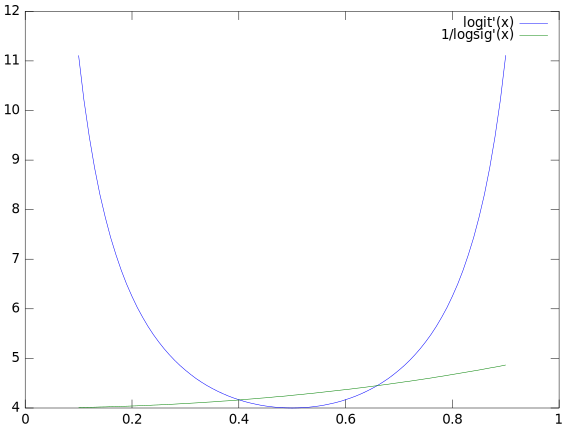
\includegraphics[scale=0.45]{logsig}
}{
\caption{${f^{(1)^{-1}}}'$ i $\frac{1}{f'^{(1)}}$ dla $logsig(x)$\label{fig:finvd2}}%
}
\end{floatrow}
\end{figure}


Eksperymenty na zbiorze DJI wykazały, że bez tej poprawki nie jest możliwe w przypadku losowej inicjalizacji $z_{ks}$ osiągnięcie tej samej wartości MSE co dla $z_{ks}$ inicjalizowanego wyjściami warstwy ukrytej. Przy wielokrotnym powtórzeniu eksperymentu (10 losowych sieci, 10 losowych wartości $z_{ks}$ dla każdej sieci, 40 iteracji procesu uczenia) uzyskane wartości MSE dla poprawionego wzoru były średnio o $10^{-5}$ lepsze przy średniej wartości rzędu $10^{-3}$.

\subsection{Zależność wag od wartości $z$}
Należy zauważyć, że wartości wag obu warstw są zależne od wartości $z_{ks}$, przez co wzór na wartość $\frac{\partial Q}{\partial z_{ks}}$ nie jest dokładny. W celu poprawy dokładności należałoby dodać do wzoru wartości $\frac{\partial w_n}{\partial z_{ks}}$, jednak ich wyznaczenie w zależności od $s$ byłoby problematyczne - wynikają z rozwiązania układu równań liniowych.

\section{Problem danych wejściowych niewielkiego wymiaru}
Dla zbioru danych regresji rozmiar pojedynczej próbki wynosił $I = 1$, optymalna ilość neuronów ukrytych $K = 5$. W trakcie uczenia sieci neuronowych metodą wrażliwościową nie udało się uzyskać dobrej jakości regresji dla optymalnej liczby neuronów, natomiast było to możliwe dla $K = 20$. Wynika to bezpośrednio z procedury uczenia metodą wrażliwościową. Dla danych wymiaru $I = 1$, dla ustalonego neuronu ukrytego $\hat{k}$, wartości $z_{\hat{k}s}$ powinny odzwierciedlać wykres funkcji aktywacji tego neuronu. Tymczasem optymalizacja $z_{\hat{k}s}$ względem oczekiwanych wartości $d_{\hat{k}s}$ powoduje, że wartości $z_{\hat{k}s}$ są rozproszone. Teoretycznie, składnik błędu $Q^{(1)}$ powinien pełnić funkcję regularyzacji, zapewniając że wartości $z_{\hat{k}s}$ zostaną uformowane w wykres funkcji aktywacji $f^{(1)}_{\hat{k}}$. W praktyce jednak na rozpatrywanym zbiorze danych regularyzacja nie zachodziła, zarówno w przypadku losowej inicjalizacji $z_{ks}$ jak i inicjalizacji wartościami wyjściowymi warstwy ukrytej. Sieć neuronowa uczyła się bardzo dobrze wyliczać wartości $y_{js}$ na podstawie $z_{ks}$, uzyskując bardzo niski błąd $MSE(z_{ks})$, natomiast nie była w stanie otrzymać tychże wartości $z_{ks}$ na podstawie wejść $x_{is}$, przez co rzeczywisty błąd sieci: $MSE(x_{is})$ utrzymywał się na wysokim poziomie.

\underline{Hipoteza}: dla danych niewielkiego wymiaru metoda wrażliwościowa nie gwarantuje uzyskania optymalnej struktury sieci. Przy większej ilości neuronów ukrytych możliwe jest uzyskanie dobrej jakości klasyfikacji/regresji, jednakże zwiększa to ryzyko uzyskania klasyfikatora o mniejszej zdolności do generalizacji (o większej wariancji).


\section{Podsumowanie}
Metoda wrażliwościowa pozwala na nauczenie sieci neuronowej w niewielkiej ilości iteracji oraz stosunkowo małym nakładem obliczeniowym. Dodatkowo, pozwala ona na lepsze zrozumienie wpływu poszczególnych neuronów warstwy ukrytej na otrzymany model poprzez analizę wrażliwości. Metoda została przez autorów przetestowana z dobrym skutkiem m.in. na znanym zbiorze MNIST, co świadczy o jej przydatności do rozwiązywania praktycznych zadań klasyfikacji i regresji. Przyspieszenie obliczeń dla podstawowego modelu sieci neuronowej daje potencjalną możliwość wykorzystania tej metody w bardziej złożonych modelach neuronowych. W szczególności szybsze obliczenia mogłyby być istotne w przypadku takich modeli jak sieci rekurencyjne, rekursywne, nieliniowe PCA czy pamięci autoasocjacyjne typu RAAM.

Metoda wrażliwościowa nie jest jednak w stanie nauczyć sieci o optymalnej architekturze w przypadku danych wejściowych o niewielkim wymiarze. Nie są znane warunki określające minimalny rozmiar danych wejściowych gwarantujący poprawne działanie metody. Nie jest też znana ilość nadmiarowych neuronów ukrytych która musi zostać użyta dla danych o zbyt małym wymiarze. Sprawia to, że metoda wrażliwościowa jest mniej pewna niż wiodące metody uczenia sieci neuronowych: LM, BFGS, choć w pewnych warunkach pozwala na znacznie szybsze nauczenie sieci neuronowej. W przypadku analizy takich danych, metoda wrażliwościowa powinna być stosowana z ostrożnością, zwłaszcza wobec komentarza autora, który stwierdza że w przypadku trafienia w minimum lokalne błędu $Q$, metoda ta nie potrafi z niego wyjść~\cite{castillo2006very}.

\bibliography{bib/sensitivity,bib/fnn}
\bibliographystyle{ieeetr}
\end{document}
